\subsection{Überprüfung der Stabilität}
\subsection{Resonator mit zwei gekrümmten Spiegeln\label{sec:curved}}
Durch Einsetzen von \eqref{eq:StabCurved} ($r_1 = r_2 = \SI{1.400}{\metre}$) in die Stabilitätsbedinung \eqref{eq:Stabilitat} ergibt sich, dass der Resonator optisch stabil ist, wenn für die Länge $L$ der Resonators gilt $\SI{0}{\metre}\leq L<\SI{2.800}{\metre}$. Dieser Bereich ist in Abbildung \ref{fig:curved} blau hinterlegt. Die minimale bzw. maximale Länge des Resonators, vorgegeben durch die Versuchsanordnung sind durch die roten Linien gekennzeichnet. Im gesamten möglichen Bereich ist der Aufbau eines stabilen Lasers möglich, wie die eingezeichneten Messwerte aus Tabelle \ref{tab:curv} belegen.
\begin{table}
    \centering
    \caption{Resonatorlänge und dazu gemessene Intensität bei einem Resonator mit zwei konkaven Spiegeln}
    \label{tab:curv}
    \sisetup{parse-numbers=false}
    \begin{tabular}{
	S[table-format=1.2]
	S[table-format=3.0]
	}
	\toprule
	{$L \ / \ \mathrm{in} \si{\metre}$}		& {$I \ / \ \si{\micro\ampere}$}		\\ 
	\midrule
    0.6 & 177.0 & 0.3 \\
0.8 & 440.0 & 0.8 \\
0.9 & 530.0 & 0.9 \\
1.1 & 530.0 & 0.9 \\
1.2 & 350.0 & 0.6 \\
1.4 & 330.0 & 0.6 \\
1.6 & 440.0 & 0.8 \\
1.7 & 570.0 & 1.0 \\
1.9 & 500.0 & 0.9 \\
2.1 & 450.0 & 0.8 \\

    \bottomrule
    \end{tabular}
    \end{table}

\begin{figure}[h!]
	\centering
	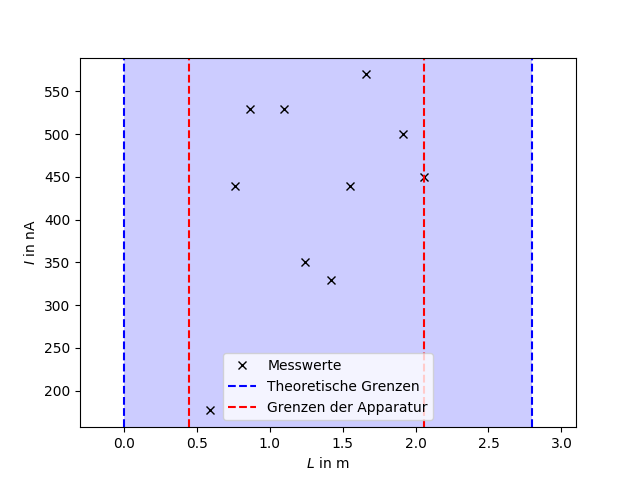
\includegraphics[width=.6\textwidth]{PlotCurved2.png}
	\caption{Veranschaulichung der Stabilitätsbedingung für einen Resonator mit zwei gekrümmten Spiegeln}
	\label{fig:curved}
\end{figure}
\clearpage
\subsection{Resonator mit einem gekrümmten und einem planaren Spiegel}
Das Vorgehen ist hier analog zu \ref{sec:curved}. Dieses Mal wird \eqref{eq:StabFlat} ($r_1 = \SI{1.400}{\metre}, r_2\rightarrow\infty$) in \eqref{eq:Stabilitat} eingesetzt und ergibt eine stabile Resonatorlänge $L$ für $\SI{0}{\metre}\leq L<\SI{1.400}{\metre}$. Der stabile Bereich ist wieder blau hinterlegt und die untere Grenze, die durch die Länge der Kammer des Lasermediums bedingt ist, ist wiederum als rote Linie eingezeichnet. Die Messwerte aus Tabelle \ref{tab:flat} decken hier nicht den ganzen möglichen Bereich ab, denn bei einer Resonatorlänge $L>\SI{0.98}{\metre}$ kann der Laser nicht mehr zum Lasen gebracht werden.
\begin{table}
    \centering
    \caption{Resonatorlänge und dazu gemessene Intensität bei einem Resonator mit einem flachen und einem konkaven Spiegel}
    \label{tab:flat}
    \sisetup{parse-numbers=false}
    \begin{tabular}{
	S[table-format=1.2]
	S[table-format=3.0]
	}
	\toprule
	{$L \ / \ \mathrm{in} \si{\metre}$}		& {$I \ / \ \si{\micro\ampere}$}		\\ 
	\midrule
    0.5 & 20.0  & 0.1 \\
0.6 & 20.0  & 0.1 \\
0.7 & 39.0  & 0.3 \\
1.0 & 95.0  & 0.6 \\
0.9 & 104.0 & 0.7 \\
1.0 & 150.0 & 1.0 \\

    \bottomrule
    \end{tabular}
    \end{table}

\begin{figure}[h!]
	\centering
	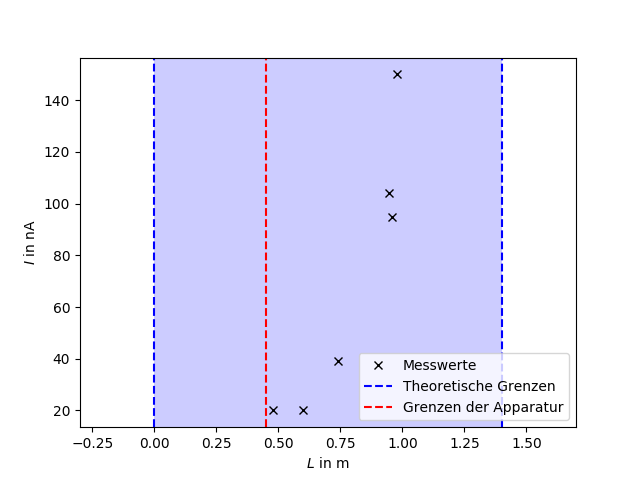
\includegraphics[width=.6\textwidth]{PlotFlat2.png}
	\caption{Veranschaulichung der Stabilitätsbedingung für einen Resonator mit einem gekrümmten und einem planaren Spiegel}
	\label{fig:flat}
\end{figure}